\documentclass{beamer}
\usepackage{relsize}
\usepackage{color}

\usepackage{listings}
\usetheme{CambridgeUS}
%\usepackage{beamerthemesplit} % new
\usepackage{enumitem}
\usepackage{amsmath}                    % See geometry.pdf to learn the layout options.
\usepackage{amsthm}                   % See geometry.pdf to learn the layout options. There
\usepackage{amssymb}                    % See geometry.pdf to learn the layout options.
\usepackage[utf8]{inputenc}
\usepackage{graphicx}
\usepackage[english,bulgarian]{babel}
\usepackage{tikz}


\usepackage{caption}

\usetheme{CambridgeUS}
\usecolortheme{crane}

\lstset{language=C++,
                basicstyle=\ttfamily,
                keywordstyle=\color{blue}\ttfamily,
                stringstyle=\color{red}\ttfamily,
                commentstyle=\color{green}\ttfamily,
                morecomment=[l][\color{magenta}]{\#}
}

\newtheorem{mydef}{Дефиниция}[section]
\newtheorem{lem}{Лема}[section]
\newtheorem{thm}{Твърдение}[section]

\DeclareMathOperator{\restrict}{\upharpoonright}

\setitemize{label=\usebeamerfont*{itemize item}%
  \usebeamercolor[fg]{itemize item}
  \usebeamertemplate{itemize item}}

\setbeamercovered{transparent}

\captionsetup{font=tiny} 

\begin{document}
\title[Функции]{Дефиниране на функции: Образци, гардове, рекурсия}
\frame{\titlepage}

\section{Функции}
\subsection{Образци}


\begin{frame}[fragile]
  \frametitle{Съпоставяне на образци (Pattern Matching)}

\begin{itemize}
  \item Литерали: разглеждане на случаи
  \begin{lstlisting}[basicstyle=\small]
    fib 0 = 1
    fib 1 = 1 
  \end{lstlisting}
  \item Променливи: винаги успешно съпоставяне
  \begin{lstlisting}[basicstyle=\small]
    fib n = fib (n-2) + fib (n-1)
  \end{lstlisting}
  \item Празни образци: винаги успешно съпоставяне
  \begin{lstlisting}[basicstyle=\small]
    const5 _ = 5
  \end{lstlisting}
\end{itemize}

\end{frame}


\begin{frame}[fragile]
  \frametitle{Съпоставяне на n-торки}

\begin{itemize}
  \item Достъп до елементите на n-торка
  \begin{lstlisting}[basicstyle=\small]
    take1 (a,_,_) = a

    >take("Ivan Ivanov", 25, "Sofia")
    "Ivan Ivanov"
  \end{lstlisting}
\end{itemize}

\end{frame}


\begin{frame}[fragile]
  \frametitle{Съпоставяне на списъци}

  Има само два вида списъци:
\begin{itemize}
  \item Празен списък
  \begin{lstlisting}[basicstyle=\small]
    mylen [] = 0
  \end{lstlisting}
  \item Непразен списък (има глава и опашка)
  \begin{lstlisting}[basicstyle=\small]
    mylen (x:xs) = 1 + mylen xs
  \end{lstlisting}
  \item Стойността на главата не ни интересува
  \begin{lstlisting}[basicstyle=\small]
    mylen (_:xs) = 1 + mylen xs
  \end{lstlisting}
  \item Фиксирани списъци
  \begin{lstlisting}[basicstyle=\small]
    sum3 [a,b,c] = a+b+c
  \end{lstlisting}
  \item Извличане на повече елементи
  \begin{lstlisting}[basicstyle=\small]
    progression [] = True
    progression [x] = True
    progression (x:y:xs) = x <= y && progression (y:xs)
  \end{lstlisting}
 
\end{itemize}

\end{frame}


\begin{frame}[fragile]
  \frametitle{Гардове: още един вид разклонение}

  \begin{lstlisting}[basicstyle=\small]
    quadrant (x,y) 
      | x > 0 && y > 0 = 1
      | x < 0 && y > 0 = 2
      | x < 0 && y < 0 = 3
      | x > 0 && y < 0 = 4
      | otherwise = 0
  \end{lstlisting}


\end{frame}



\begin{frame}[fragile]
  \frametitle{Рекурсия със списъци}


  \begin{itemize}
    \item Намиране на сума, максимум, търсене, повторения, скаларно произведение
    \item Намиране на префикс, суфикс, обръщане
    \item Намиране на обединение, сечение, общ префикс, сортирано сливане
    \item Намиране на най-често срещан елемент
  \end{itemize}  

\begin{center}
  \begin{figure}
    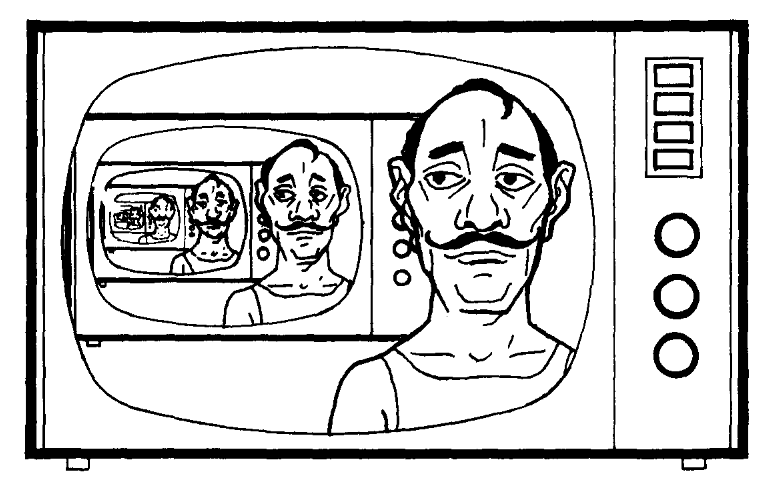
\includegraphics[width=4.0cm]{images/rec_wirt}  
    \caption{Рекурсия според Никлаус Вирт[1]}
  \end{figure}
  
\end{center}
\end{frame}

\begin{frame}[fragile]
  \frametitle{where: let наобратно}
  \begin{lstlisting}[basicstyle=\small]
    mostcommon [x] = (x,1)
    mostcommon (x:xs) 
        | count x xs == n = (x,n+1)
        | otherwise = (y,n)
        where (y,n) = mostcommon xs    
  \end{lstlisting}
\end{frame}



\begin{frame}[fragile]
  \frametitle{Цитирани източници}

  \relscale{0.5}
    [1] Wirth.,N.,``Algorithms + Data Structures = Programs'', Prentice Hall,1976
\end{frame}

\begin{frame}[fragile]
    \frametitle{}
  
  \centerline{Благодаря за вниманието!}
\newcommand{\license}[1]{
  \begin{tikzpicture}[remember picture,overlay]
      \node[xshift=0mm,yshift=13mm,anchor=south east] at (current page.south east)
      {\tiny{Материалите са разработени от Калин Георгиев за курсовете по програмиране на ФМИ, СУ}};
      \node[xshift=0mm,yshift=10mm,anchor=south east] at (current page.south east)
      {\tiny{Creative Commons Attribution-NonCommercial-ShareAlike 4.0 International}};
      \node[xshift=0mm,yshift=5mm,anchor=south east] at (current page.south east){%
      \includegraphics[width=30mm]{{#1}/license}};
    \end{tikzpicture}
}
\license{../../..}
 
\end{frame}  


\end{document}



\begin{columns}[t]
  \begin{column}{0.2\textwidth}

\relscale{0.63}
\begin{lstlisting}
\end{lstlisting}
\relscale{1}

  \end{column}
  \begin{column}{0.8\textwidth}

  \end{column}
\end{columns}


